%-----------------------------------------------------------------------------%
\chapter{\babTiga}
\label{bab:3}
%-----------------------------------------------------------------------------%
Bab ketiga ini menjelaskan tentang rancangan dan metodologi yang penulis lakukan dalam penelitian ini. Sub-bab \ref{3.1} menjelaskan mengenai gambaran umum terkait bagaimana teknik untuk memanfaatkan NLI untuk meningkatkan performa suatu sistem tanya jawab. Sub-bab \ref{3.2} menjelaskan mengenai tahapan penelitian yang akan penulis lakukan. Sub-bab \ref{3.3} menjelaskan mengenai eksplorasi \emph{dataset} yang penulis lakukan. Sub-bab \ref{3.4} menjelaskan pelatihan model dan alur eksperimen yang dilakukan. Sub-bab \ref{3.5} lalu menjelaskan teknik evaluasi dan analisis hasil yang digunakan setiap metode.

%-----------------------------------------------------------------------------%
\section{Pemanfaatan NLI Untuk Sistem Tanya Jawab}
\label{3.1}
%-----------------------------------------------------------------------------%
Sebagai pembuka dari bagian metodologi ini, penelitian ini ditujukan untuk mengetahui apakah performa sistem tanya jawab berbahasa Indonesia akan lebih baik dengan memanfaatkan NLI dan jenis-jenis pertanyaan apa saja yang lebih baik dengan memanfaatkan NLI. Untuk data yang penulis gunakan dapat terbagi menjadi dua bagian, data NLI dan data sistem tanya jawab. Untuk data NLI, penulis hanya menggunakan satu \emph{dataset}, yaitu: \emph{dataset} IndoNLI \citep{mahendra-etal-2021-indonli}. Alasan menggunakan \emph{dataset} ini adalah: karena topik utama penelitian ini adalah melanjutkan topik penelitian \citet{mahendra-etal-2021-indonli} terkait pemanfaatan \emph{dataset} IndoNLI pada beragam tugas (\emph{task}) bidang NLP, salah satunya adalah sistem tanya jawab (\emph{question answering}). Kemudian, untuk data sistem tanya jawab, penulis menggunakan tiga \emph{dataset} sebagai tolak ukur (\emph{benchmark}) dari evaluasi sistem tanya jawab yang penulis rancang, yaitu: \emph{dataset} SQuAD-ID \citep{muis2020sequencetosequence}, TyDi-QA-ID \citep{cahyawijaya-etal-2021-indonlg}, IDK-MRC \citep{putri-oh-2022-idk}. Alasan menggunakan ketiga \emph{dataset} ini adalah: karena menurut penulis, ketiga \emph{dataset} ini merupakan \emph{dataset} terbaik untuk dijadikan tolak ukur (\emph{benchmark}) sistem tanya jawab berbahasa Indonesia. Penggunaan tiga \emph{dataset} sekaligus juga penulis tujukan agar sistem tanya jawab dapat menangkap pola-pola variasi beragam \emph{dataset} sistem tanya jawab, sehingga sistem tanya jawab buatan penulis berhasil menggeneralisasikan pola-pola tersebut untuk menghasilkan prediksi jawaban yang lebih kokoh (\emph{robust}).

Kemudian, ada tiga model yang penulis gunakan pada penelitian ini, yaitu: \texttt{indobert-base-uncased}, \texttt{indobert-large-p2}, \texttt{xlm-roberta-large}. Pemilihan ketiga model tersebut didasari oleh dua hal utama, yaitu: keandalan model untuk menyelesaikan permasalahan bahasa Indonesia, karena model \texttt{indobert-base-uncased} dan model \texttt{indobert-large-p2} dilatih pada korpus berbahasa Indonesia berskala besar \citep{koto2020indolem, cahyawijaya-etal-2021-indonlg}, dan model \texttt{xlm-roberta-large} dilatih pada korpus banyak bahasa (\emph{multi-lingual}) \citep{conneau2020unsupervised}; kemudian, alasan kedua adalah sebagai pembeda (\emph{distinguisher}) antar model, karena model \texttt{indobert-base-uncased} memiliki ukuran yang lebih kecil (jumlah parameternya) dibandingkan dengan model \texttt{indobert-large-p2}, dan model \texttt{indobert-large-p2} memiliki ukuran yang lebih kecil (korpus latihnya) dibandingkan dengan model \texttt{xlm-roberta-large}.

Terakhir, metode yang penulis gunakan pada penelitian ini secara umum dapat dibagi dua, yaitu: \emph{intermediate task transfer learning} dan \emph{task recasting} sebagai verifikator. Pemilihan dua metode tersebut didasari oleh kemudahan memahami alur pemanfaatan NLI-nya, dikarenakan kedua metode tersebut merupakan metode yang masuk akal, mudah dipahami, dan \emph{straight to the point}, sehingga cara memanfaatkan NLI-nya tergambar dengan jelas di kepala. Untuk metode \emph{intermediate task transfer learning} penulis mengikuti teknik yang digunakan oleh \citeauthor{pruksachatkun-etal-2020-intermediate}, yaitu dengan memecah tugasnya menjadi dua, yaitu: \emph{intermediate task} dan \emph{target task}. Kemudian, untuk metode \emph{task recasting}  sebagai verifikator, penulis mengikuti teknik yang digunakan oleh \citeauthor{chen-etal-2021-nli-models}, yaitu dengan melakukan penyaringan (\emph{filtering}) prediksi jawaban dengan parameter hasil label NLI-nya. Pada penelitian ini, \emph{intermediate task} yang dipilih adalah \emph{sequence classification task} dengan menggunakan \emph{dataset} IndoNLI, dan \emph{target task} yang dipilih adalah \emph{question answering task} dengan menggunakan \emph{dataset} SQuAD-ID, TyDi-QA-ID, dan IDK-MRC. Untuk alur eksperimen tahap ini, akan dijelaskan pada sub-bab selanjutnya. Pada penelitian ini, prediksi jawaban oleh model \emph{question answering} tidak diganggu sama sekali, setelah prediksi jawaban didapatkan, baru dilakukan penyaringan (\emph{filtering}) prediksi jawabannya. Untuk alur eksperimen tahap ini, akan dijelaskan pada sub-bab selanjutnya. Bab metodologi ini akan berfokus kepada gambaran umum dari penelitian ini.

%-----------------------------------------------------------------------------%
\section{Tahapan Penelitian}
\label{3.2}
%-----------------------------------------------------------------------------%
Pada sub-bab ini, akan dijelaskan mengenai tahapan penelitian yang penulis gunakan pada penelitian ini. Tahapan penelitian yang penulis lakukan adalah sebagai berikut:

\begin{itemize}
    
    \item \textbf{Pencarian \emph{dataset}, model, dan metode}: Pada tahap ini penulis melakukan pencarian untuk memilih emph{dataset}, model, dan metode eksperimen apa saja yang akan digunakan dalam penelitian ini. Tahap ini meliputi pemilihan emph{dataset} dan model yang akan digunakan untuk tiap metode dan penjelasan metode yang dipakai untuk penelitian. Kemudian, untuk metode penelitian, penulis memutuskan untuk menggunakan tiga metode eksperimen, yaitu: \emph{intermediate-task transfer learning} dan \emph{task recasting} dengan IndoNLI sebagai verifikator. Hasil dari tahap ini adalah emph{dataset} yang akan digunakan pada tahap selanjutnya.

    \item \textbf{Eksplorasi \emph{dataset} (EDA) sistem tanya jawab}: Pada tahap ini penulis melakukan eksplorasi dari \emph{dataset} sistem tanya jawab yang telah dipilih sebelumnya. Eksplorasi \emph{dataset} (EDA) dilakukan dengan bertujuan untuk mengerti karakteristik dari suatu \emph{dataset} sistem tanya jawab yang sedang diproses. Proses EDA ini penulis contoh dari penelitian \citep{nguyen-etal-2020-vietnamese, rajpurkar-etal-2016-squad}. Semua proses EDA dilakukan secara otomatis (via kode Python), kecuali proses \emph{reasoning type}; pada proses \emph{reasoning type} penulis berkolaborasi dengan seorang mahasiswa Tugas Akhir (TA) Fasilkom lainnya untuk menganotasikan \emph{reasoning type} 100 data per \emph{test set} dari suatu \emph{dataset} sistem tanya jawab. Dari dua iterasi proses anotasi, didapatkan hasil \emph{cohen kappa} sebesar 0.91 untuk \emph{dataset} SQuAD-ID, hasil \emph{cohen kappa} sebesar 0.92 untuk \emph{dataset} TyDI-QA-ID, hasil \emph{cohen kappa} sebesar 0.96 untuk \emph{dataset} IDK-MRC; dan dari skor-skor tersebut, dapat diinterpretasikan bahwa: anotasi mencapai kesepakatan hampir sempurna (\emph{near perfect agreement}), sehingga hasil anotasi reliabel \emph{reasoning type} untuk digunakan sebagai bahan evaluasi dan analisis kedepannya. 

    \item \textbf{\emph{Training sequence classification task}}: Pada tahap ini, penulis melakukan \emph{training} terlebih dahulu untuk \emph{sequence classification task} untuk belajar terkait \emph{natural language inference}. \emph{Training} dilakukan dengan menggunakan masing-masing tiga model, dan tiga \emph{dataset}. Pada sub-bab ini akan ditekankan terkait \emph{dataset} yang penulis gunakan. \emph{Dataset} yang penulis gunakan dalam \emph{training sequence classification task} ini dibagi tiga, yaitu: IndoNLI-\emph{basic}, IndoNLI-\emph{translated}, IndoNLI-\emph{augmented}. Dimana, IndoNLI-\emph{basic} merupakan data NLI berbahasa Indonesia yang dianotasikan oleh manusia, kemudian IndoNLI-\emph{translated} merupakan \emph{dataset} MNLI yang diterjemahkan ke bahasa Indonesia, lalu IndoNLI-\emph{augmented} merupakan gabungan dari IndoNLI-\emph{basic} dan IndoNLI-\emph{translated}. Untuk alur penelitian tahapan ini sangat sederhana, yaitu: mencoba satu-satu setiap model \& \emph{dataset} IndoNLI-nya, dan cari hasil yang terbaik dari hasil \emph{training}-nya. Dimana, hasil yang terbaik itu akan disuplai ke metode \emph{intermediate-task transfer learning} dan \emph{task recasting}. Tahapan ini berguna untuk menyuplai model untuk \emph{intermediate task} dan model untuk verifikator pada metode penelitian saat ini. Untuk alur dan implementasi lebih jelasnya, dapat dilihat pada bab selanjutnya.

    \item \textbf{\emph{Training baseline question answering system}}: Pada tahapan ini, eksperimen dilakukan dengan sangat sederhana. Dimana, model yang telah dipilih sebelumnya dilatih dengan \emph{question answering task}, dengan tiga \emph{dataset} yang berbeda. Tahapan ini digunakan sebagai acuan awal, apakah metode-metode pemanfaatan IndoNLI berhasil meningkatkan atau menurunkan performa sistem tanya jawab yang orisinil, tanpa penambahan metode apapun. Terakhir, menyimpan keseluruhan hasil eksperimen ini untuk nantinya akan dilakukan evaluasi dan analisis hasil eksperimen. Tahapan ini berguna untuk menyuplai model untuk acuan hasil awal/dasar dari \emph{question answering} tanpa pemanfaatan NLI sama sekali, atau dalam kata lain sebagai model untuk \emph{target task} dan model untuk prediksi jawaban yang nantinya akan dilakukan verifikasi pada metode penelitian saat ini. Untuk alur dan implementasi lebih jelasnya, dapat dilihat pada bab selanjutnya.
    
    \item \textbf{Pelatihan model dan eksperimen}: Pada tahap ini penulis melakukan pelatihan model dan eksperimen-eksperimen berdasarkan data, model, dan metode yang sudah dipilih pada tahap sebelumnya. Tahap ini meliputi pelatihan model yang akan digunakan untuk tiap metode. Hasil dari tahap ini adalah model yang sudah dilatih berdasarkan metode yang telah dipilih yang menghasilkan hasil eksperimen untuk dilakukan analisis pada tahap berikutnya.

    \item \textbf{Evaluasi dan analisis hasil}: Pada tahap ini penulis melakukan evaluasi dan analisis berdasarkan hasil yang sudah didapatkan pada tahap sebelumnya. Tahap ini meliputi pemilihan metrik evaluasi yang digunakan untuk setiap metode eksperimen penelitian.

\end{itemize}

%-----------------------------------------------------------------------------%
\section{Eksplorasi \emph{Dataset} (EDA) Sistem Tanya Jawab}
\label{3.3}
%-----------------------------------------------------------------------------%
Pada sub-bab ini, akan dijelaskan mengenai eksplorasi \emph{dataset} (EDA) sistem tanya jawab yang telah dipilih sebelumnya. Eksplorasi yang penulis lakukan sama persis dengan apa yang telah dilakukan \citet{nguyen-etal-2020-vietnamese} dan \citet{rajpurkar-etal-2016-squad} pada tahapan ekplorasi \emph{dataset machine reading comprehension} untuk bahasa Vietnam. Ada beberapa bagian yang penulis jadikan bahan eksplorasi, antara lain:

\begin{itemize}

    \item \emph{Overview Statistics}

        \begin{itemize}
            \item Banyaknya artikel.
            \item Banyaknya konteks.
            \item Banyaknya pertanyaan.
            \item Banyaknya jawaban yang eksis.
            \item Banyaknya jawaban yang tidak eksis.
            \item Rata-rata panjang kata dari konteks.
            \item Rata-rata panjang kata dari pertanyaan.
            \item Rata-rata panjang kata dari jawaban.
            \item Ukuran kosakata (\emph{Vocabulary size}).
        \end{itemize}

    \item \emph{Length-based analysis}

        \begin{itemize}
            \item Rincian distribusi panjang kata dari konteks.
            \item Rincian distribusi panjang kata dari pertanyaan.
            \item Rincian distribusi panjang kata dari jawaban.
        \end{itemize}
        
    \item \emph{Type-based analysis}

        \begin{itemize}
            \item \emph{Question type}.
            \item \emph{Reasoning type}.
            \item \emph{Answer type}.
        \end{itemize}

\end{itemize}

Untuk arti dari \emph{question type}, sederhananya adalah tipe pertanyaan, dapat dibagi menjadi delapan bagian, antara lain: pertanyaan apa, pertanyaan siapa, pertanyaan kapan, pertanyaan dimana, pertanyaan mengapa, pertanyaan bagaimana, pertanyaan berapa, pertanyaan lainnya. Bagian ini dilakukan secara manual, dengan mendeteksi kalimat tanya yang terdapat pada pertanyaan via kode Python.

Untuk arti dari masing-masing \emph{reasoning type}, menurut \citeauthor{9247161}, arti dari WM (\emph{Word Matching}) adalah \emph{token} pertanyaan yang ini persis cocok dengan \emph{token} dalam konteks, kemudian arti dari PP (\emph{Paraphrasing}) adalah kalimat pertanyaan yang merupakan parafrase dari satu kalimat dalam konteks, lalu arti dari SSR (\emph{Single-sentence reasoning}) adalah kalimat jawaban yang ditarik kesimpulannya dari satu kalimat dalam konteks, kemudian arti dari MSR (\emph{Multi-sentence reasoning}) adalah kalimat jawaban yang ditarik kesimpulannya dari banyak kalimat dalam konteks, terakhir arti dari AoI (\emph{Ambiguous or insufficient}) adalah kalimat pertanyaan yang memiliki banyak jawaban atau jawaban tidak ditemukan dalam konteks. Bagian ini dilakukan secara manual, dengan melakukan kolaborasi anotasi dengan mahasiswa Tugas Akhir lainnya.

Untuk arti dari masing-masing \emph{answer type} yang digunakan pada penelitian ini, sudah penulis sertakan di Lampiran \ref{Lampiran Terkait Penjelasan: 7.2}. Bagian ini dilakukan secara otomatis, dengan menggunakan model \emph{entity-named recognition} berbahasa Indonesia dengan model \href{https://huggingface.co/cahya/xlm-roberta-base-indonesian-NER}{\texttt{cahya/xlm-roberta-base-indonesian-NER}}, penulis menggunakan model tersebut karena memiliki ketersediannya pada repositori Hugging Face dan memiliki performa yang baik.

Properti-properti di atas yang akan menjadi bahan evaluasi dan analisis penelitian ini yang telah tertuang pada sub-bab \ref{1.2} dan sub-bab \ref{1.3} yang telah dituliskan di bab sebelumnya. Penggunaan properti-properti di atas ditujukan untuk mendalami dan menambah wawasan terkait \emph{dataset} sistem tanya jawab.

%-----------------------------------------------------------------------------%
\section{Pelatihan Model dan Eksperimen}
\label{3.4}
%-----------------------------------------------------------------------------%
Pada sub-bab ini, akan dijelaskan mengenai pelatihan model dan eksperimen yang penulis lakukan pada pada penelitian ini. 

%-----------------------------------------------------------------------------%
\subsection{\emph{Intermediate-Task Transfer Learning}}
\label{3.4.1}
%-----------------------------------------------------------------------------%

\begin{figure}[h]
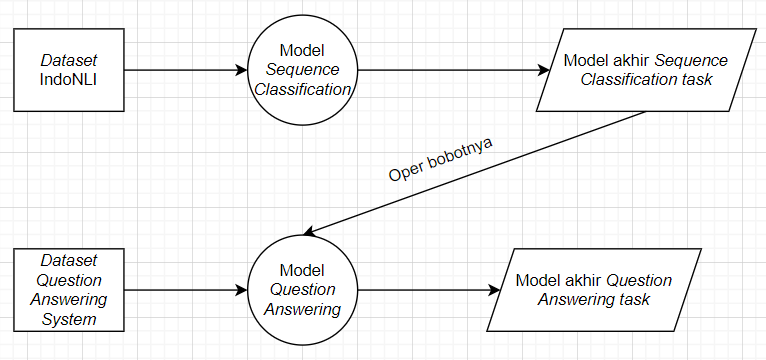
\includegraphics[width=\linewidth]{assets/pics/alur1.png}
\centering
\caption{Visualisasi grafik pada metode \emph{intermediate-task transfer learning}.}
\end{figure}

Alur penelitian tahapan \emph{intermediate-task transfer learning} yang penulis lakukan adalah sebagai berikut:

\begin{itemize}

    \item Model yang telah dilatih pada \emph{task} \emph{sequence classification}, kemudian bobot (\emph{weight}) dari hasil latih tersebut disimpan terlebih dahulu.

    \item Kemudian, model-model baru akan diinisiasikan dengan \emph{task} \emph{question answering} sebagai \emph{target task}-nya.

    \item Namun, bobot model untuk \emph{task} \emph{question answering} didapatkan dari bobot model \emph{task} \emph{sequence classification} yang sebelumnya disimpan. Disini, penulis membuat dua alur, pertama, apakah bobot dari  \emph{task} \emph{sequence classification} akan dilatih ulang semua \emph{layer}-nya atau hanya akan dilatih ulang pada \emph{layer} klasifier-nya saja \citep{lee2019elsa}.

    \item Terakhir, menyimpan keseluruhan hasil eksperimen ini untuk nantinya akan dilakukan evaluasi dan analisis hasil eksperimen.

\end{itemize}

Untuk alur dan implementasi lebih jelasnya, dapat dilihat pada bab selanjutnya.

%-----------------------------------------------------------------------------%
\subsection{\emph{Task Recasting} Dengan NLI Sebagai Verifikator}
\label{3.4.2}
%-----------------------------------------------------------------------------%

\begin{figure}[h]
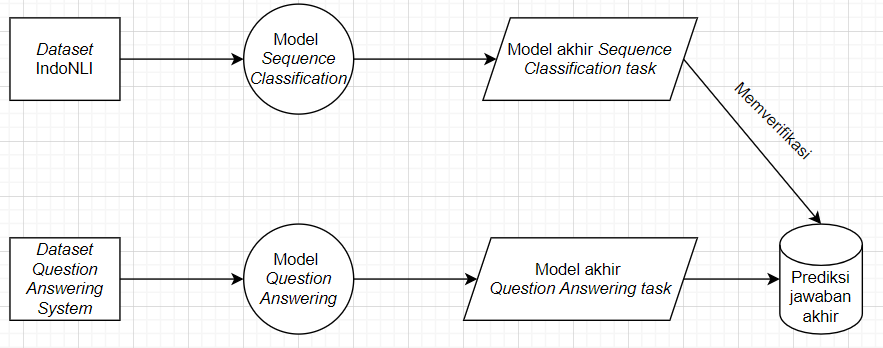
\includegraphics[width=\linewidth]{assets/pics/alur2.png}
\centering
\caption{Visualisasi grafik pada metode \emph{task recasting} dengan NLI sebagai verifikator.}
\end{figure}

Alur penelitian tahapan \emph{task} recasting dengan NLI sebagai verifikator yang penulis lakukan adalah sebagai berikut:

\begin{itemize}
    
    \item Menyiapkan model-model yang telah telah dilatih pada \emph{task} \emph{sequence classification} sebagai verifikator parameter NLI pada \emph{task} \emph{question answering}-nya.

    \item Kemudian, model-model baru diinisiasikan dengan \emph{task} \emph{question answering} sebagai prediktor dari \emph{dataset} \emph{question answering system}-nya.
    
    \item Setelah dilatih, model-model \emph{task} \emph{question answering} tersebut memprediksi jawaban dari konteks (dari \emph{test set}) yang sudah tersedia.
    
    \item Kemudian, pada tahap ini dilakukan perubahan struktur hasil prediksi sistem tanya jawab menjadi struktur yang dapat dinilai berdasarkan parameter label NLI-nya, pengubahan ini dapat dilakukan dengan melakukan perubahan format kalimat atau bisa disebut dengan \emph{smoothing}. \emph{Smoothing} sendiri merupakan istilah yang digunakan untuk menyebutkan pengubahan dari pasangan jawaban dan pertanyaan menjadi hipotesis deklaratif dalam sudut pandang NLI. Pengecekan label NLI-nya menggunakan model yang telah dilatih dengan \emph{task} \emph{sequence classification} sebelumnya. Selanjutnya, terdapat berbagai parameter, meliputi:
    
    \begin{itemize}
    \item Jumlah iterasi maksimum: berapa kali akan dilakukan iterasi pencarian kemungkinan pilihan jawaban terbesar bila jawaban tidak sesuai dengan label yang dipilih pada tipe \emph{filtering}.
    
    \item Tipe \emph{filtering}:
    \begin{itemize}
        \item Bila \texttt{entailment\char`_only} dipilih, maka prediksi jawaban hanya akan diterima dan dijadikan prediksi jawaban akhir bila label NLI-nya merupakan label \texttt{entailment}; dan akan melakukan iterasi pencarian kemungkinan pilihan jawaban terbesar bila mendapatkan label \texttt{contradiction} atau label \texttt{neutral}.
        
        \item Bila \texttt{entailment\char`_or\char`_neutral} dipilih, maka prediksi jawaban hanya akan diterima dan dijadikan prediksi jawaban akhir bila label NLI-nya merupakan label \texttt{entailment} atau label \texttt{neutral}; dan akan melakukan iterasi pencarian kemungkinan pilihan jawaban terbesar bila mendapatkan label \texttt{contradiction}. 
    \end{itemize}
    
    \item Tipe perubahan format kalimat:
    \begin{itemize}
        \item Bila memilih \texttt{replace\_first}, maka pasangan kalimat \texttt{question-answer} dan \texttt{context} akan diubah menjadi pasangan kalimat \texttt{premise-hypothesis} dengan mengubah \textbf{kata terdepan} dari \texttt{question} dengan \texttt{answer} dan menghapus tanda tanya sebagai \texttt{hypothesis}; dan \texttt{context} diubah menjadi \texttt{premise}.
        
        \item Bila memilih \texttt{replace\_question\_word}, maka pasangan kalimat \texttt{question-answer} dan \texttt{context} akan diubah menjadi pasangan kalimat \texttt{premise-hypothesis} dengan mengubah \textbf{kata tanya} dari \texttt{question} dengan \texttt{answer} dan menghapus tanda tanya sebagai \texttt{hypothesis}; dan \texttt{context} diubah menjadi \texttt{premise}.
        
        \item  Bila memilih \texttt{add\_adalah}, maka pasangan kalimat \texttt{question-answer} dan \texttt{context} akan diubah menjadi pasangan kalimat \texttt{premise-hypothesis} dengan \textbf{menghapus} \textbf{kata terdepan} dari \texttt{question}, menghapus tanda tanya, dan menambahkan \texttt{answer} diakhir \texttt{question} sebagai \texttt{hypothesis}; dan \texttt{context} diubah menjadi \texttt{premise}.
        
        \item Bila memilih \texttt{just\_concat\_answer\_and\_question}, maka pasangan kalimat \texttt{question-answer} dan \texttt{context} akan diubah menjadi pasangan kalimat \texttt{premise-hypothesis} dengan menambahkan \emph{string} \texttt{answer} setelah \texttt{question} sebagai \texttt{hypothesis}; dan \texttt{context} diubah menjadi \texttt{premise}.
        
        \item  Bila memilih \texttt{rule\_based}, maka pasangan kalimat \texttt{question-answer} dan \texttt{context} akan diubah menjadi pasangan kalimat \texttt{premise-hypothesis} dengan menyesuaikan template yang telah penulis rancang manual dengan melihat contoh-contoh data pada ketiga \emph{dataset} sistem tanya jawab yang digunakan untuk setiap tipe pertanyaan, hal tersebut sebagai \texttt{hypothesis}; dan \texttt{context} diubah menjadi \texttt{premise}.
        
        \item Bila memilih \texttt{machine\_generation\_with\_rule\_based}, maka pasangan kalimat \texttt{question-answer} dan \texttt{context} akan diubah menjadi pasangan kalimat \texttt{premise-hypothesis} dengan melakukan tipe perubahan format kalimat \textbf{\texttt{rule\_based}}, lalu dilakukan \emph{paraphrase} menggunakan model \emph{paraphraser} berbahasa Indonesia untuk "menghaluskan" kalimat, hal tersebut sebagai \texttt{hypothesis}; dan \texttt{context} diubah menjadi \texttt{premise}.
        
        \item  Bila memilih \texttt{pure\_machine\_generation}, maka pasangan kalimat \texttt{question-answer} dan \texttt{context} akan diubah menjadi pasangan kalimat \texttt{premise-hypothesis} dengan melakukan tipe perubahan format kalimat \textbf{\texttt{just\_concat\_answer\_and\_question}}, lalu dilakukan \emph{paraphrase} menggunakan model \emph{paraphraser} berbahasa Indonesia untuk "menghaluskan" kalimat agar dapat murni mendapatkan hasil yang lebih murni dari \emph{paraphraser}-nya, hal tersebut sebagai \texttt{hypothesis}; dan \texttt{context} diubah menjadi \texttt{premise}.
        
        \item Bila memilih \texttt{machine\_generation\_with\_translation}, maka pasangan kalimat \texttt{question-answer} dan \texttt{context} akan diubah menjadi pasangan kalimat \texttt{premise-hypothesis} dengan melakukan tipe perubahan format kalimat \textbf{\texttt{rule\_based}}, lalu dilakukan penerjemahan ke bahasa Inggris, kemudian dilakukan \emph{paraphrase} menggunakan model \emph{paraphraser} berbahasa Inggris untuk "menghaluskan" kalimat, terakhir, diterjemahkan lagi ke bahasa Indonesia, hal tersebut dilakukan karena lebih banyak model \emph{paraphraser} berbahasa Inggris yang jauh lebih baik daripada model \emph{paraphraser} berbahasa Indonesia; namun, bila \emph{paraphraser} bahasa Inggris gagal karena saking buruknya (atau gagal menemukan terjemahannya sama sekali) terjemahan perubahan format kalimat dari bahasa Indonesia ke bahasa Inggris (sampai bertipe NoneType), maka akan dilakukan teknik \texttt{rule\_based} saja. Hal tersebut sebagai \texttt{hypothesis}; dan \texttt{context} diubah menjadi \texttt{premise}.
    \end{itemize}
    
    \item Variasi Pengambilan Jawaban Akhir:
    \begin{itemize}
        \item Bila memilih variasi 1, maka \emph{filtering} akan dibasiskan dengan label dari hasil NLI-nya saja, bila labelnya sudah sesuai tipe \emph{filtering}, maka akan masuk sebagai jawaban prediksi akhir. Bila setelah jumlah iterasi maksimum yang sudah didefinisikan sebelumnya tetap tidak memenuhi label tipe \emph{filtering}, maka akan dijawab kosong, atau dalam kata lain model tidak dapat menjawab pertanyaan tersebut \emph{unanswerable}.
        
        \item Bila memilih variasi 2, maka \emph{filtering} akan dibasiskan dengan dengan label dan skor \emph{probability distribution} dari hasil NLI-nya, bila labelnya sudah sesuai tipe \emph{filtering} dan nilai skornya memenuhi \emph{threshold}, maka akan masuk sebagai jawaban prediksi akhir. Bila setelah jumlah iterasi maksimum yang sudah didefinisikan sebelumnya tetap tidak memenuhi label tipe \emph{filtering} dan nilai skornya masih belum memenuhi \emph{threshold}, maka akan dijawab kosong, atau dalam kata lain model tidak dapat menjawab pertanyaan tersebut \emph{unanswerable}.
        
        \item Bila memilih variasi 3, maka \emph{filtering} akan dibasiskan dengan dengan label dan skor \emph{probability distribution} dari hasil NLI-nya, bila labelnya sudah sesuai tipe \emph{filtering} dan nilai skornya memenuhi \emph{threshold}, maka akan masuk sebagai jawaban prediksi akhir. Bila setelah jumlah iterasi maksimum yang sudah didefinisikan sebelumnya tetap tidak memenuhi label tipe \emph{filtering} dan nilai skornya masih belum memenuhi \emph{threshold}, maka akan dijawab dengan skor \emph{probability distribution} yang terbesar (atau dalam kata lain, paling mendekati label yang disuplai pada tipe \emph{filtering} sebelumnya) dari iterasi pencarian jawaban yang telah dilakukan, hal ini tidak membuat model verifikasi otomatis menjawab kosong, atau dalam kata lain model masih ada kemungkinan untuk menjawab pertanyaan tersebut \emph{answerable} (bila skor \emph{probability distribution} yang terbesar bukan jawaban kosong). 
    \end{itemize}
    
    \item \emph{Threshold}: berapa batas yang masih ditolerir oleh model verifikasi, untuk menentukan \emph{confidence} yang tepat untuk suatu label yang didapatkan.
\end{itemize}
    
    \item Kemudian, dilakukan penyaringan (\emph{filtering}) jawaban, alurnya dilakukan sebagai berikut:
    
    \begin{itemize}
        
        \item Jika label hasil prediksi jawaban dari model \emph{question answering task} sudah sesuai dengan label hasil pilihan tipe \emph{filtering} di atas, maka hasil jawaban tersebut disimpan dan dikeluarkan sebagai prediksi akhir.
        
        \item Sedangkan, jika label hasil prediksi jawaban dari model \emph{question answering task} belum sesuai dengan label hasil pilihan tipe \emph{filtering} di atas, maka akan dilakukan pencarian berdasarkan hasil pilihan parameter pencarian iterasi maksimum di atas. Pencarian ini didasari dengan ide \emph{arg max} pada \emph{tensor} hasil prediksi, sehingga mencari \emph{arg max} kedua, \emph{arg max} ketiga, dan \emph{arg max} seterusnya, sesuai dengan pilihan parameter pencarian iterasi maksimum yang sudah dipilih di atas. Setiap iterasi pencarian ini, akan disimpan jawaban dan label NLI-nya. Bila sudah menemukan label dan jawaban yang sesuai dengan label hasil pilihan tipe \emph{filtering} di atas, maka hasil jawaban tersebut disimpan dan dikeluarkan sebagai prediksi final.
        
        \item Bila sampai iterasi terakhir tidak ditemukan juga hasil prediksi jawaban yang sesuai dengan label hasil pilihan tipe \emph{filtering} di atas, maka akan otomatis menyimpan jawaban kosong sebagai prediksi final atau mengambil jawaban dengan \emph{probability distribution} NLI paling mendekati label yang diinginkan pada tipe \emph{filtering} sebelumnya. Hal ini ditujukan untuk mencakup \emph{unanswerable question} yang terdapat pada tiga \emph{dataset} pilihan sistem tanya jawab penelitian ini.
        
    \end{itemize}
    
    \item Terakhir, menyimpan keseluruhan hasil eksperimen ini untuk nantinya akan dilakukan evaluasi dan analisis hasil eksperimen.

\end{itemize}

Untuk alur dan implementasi lebih jelasnya, dapat dilihat pada bab selanjutnya.

%-----------------------------------------------------------------------------%
\section{Evaluasi dan Analisis Hasil}
\label{3.5}
%-----------------------------------------------------------------------------%
Pada sub-bab ini, akan dilakukan tahapan evaluasi dan analisis hasil kedua metode itu dengan \emph{baseline}-nya (tanpa dilakukan eksperimen pemanfaatan NLI sama sekali), kemudian, metrik yang dipilih sebagai bahan evaluasi dan analisis secara umum ada dua, yaitu: \emph{exact match} (atau bisa direpresentasikan sebagai akurasi) dan skor F1 berdasarkan \emph{token} prediksi jawaban. Pemilihan kedua metrik evaluasi tersebut didasari oleh keinginan penulis untuk mencontoh \citep{rajpurkar-etal-2016-squad} dalam penggunaan metrik evaluasi sistem tanya jawab. Dengan kedua metrik tersebut, seharusnya sudah dapat terbaca penurunan ataupun peningkatan performa dari model sistem tanya jawab yang telah dirancang dan juga dapat dilihat perbandingan hasil sebelum dilakukan pemanfaatan NLI dengan hasil setelah dilakukan pemanfaatan NLI. Tahapan evaluasi dan analisis pada eksperimen ini dirancang dan ditujukan untuk mengetahui pengaruh dari suatu parameter yang dimasukkan ke dalam suatu metode pemanfaatan NLI untuk sistem tanya jawab.

Kemudian, pada penelitian ini juga akan dilakukan analisis lebih dalam demi memahami karakteristik pasangan konteks-pertanyaan-jawaban apa saja yang bisa meningkat tingkat kebenarannya karena pemanfaatan NLI ini. Untuk karakteristik yang penulis analisis, antara lain: \emph{question type}, panjang konteks, panjang pertanyaan, panjang jawaban \emph{golden truth}, \emph{answer type}, dan \emph{reasoning type}. Analisis ini secara umum akan berkisar di persentase jawaban prediksi yang benar (dihitung sebagai \emph{exact match}) dibandingkan jawaban prediksi yang salah, dengan memperhatikan karakteristik pasangan pertanyaan-jawaban-konteks.